\documentclass[a4paper,parskip]{scrartcl}
\usepackage[usenames,dvipsnames,svgnames,table]{xcolor}
\usepackage[utf8]{inputenc}
\usepackage[ngerman]{babel}
\usepackage{amsmath}
\usepackage{enumerate}
\usepackage{textcomp}
\usepackage{fancyhdr}
\usepackage[a4paper]{geometry}
\usepackage{amsthm}
\usepackage{amsfonts}
\usepackage[version=3]{mhchem}
\usepackage{graphicx}


\author{Sven Jandura} 
\title{Svens Fit Sachen}

\geometry {
  top=0.75in,
  headsep=3ex,
  bottom=0.75in,
}

\fancypagestyle{plain}{
  \fancyhf{}
  \fancyhead[L]{Sven Jandura}
  %\fancyhead[C]{} %Center
  \fancyhead[R]{Seite \thepage}
}

\renewcommand{\headrule}{\color{Black}\hrule height\headrulewidth\hfill}
\pagestyle{plain}

\let\stdsection\section\renewcommand\section{\newpage\stdsection}

\newtheorem{mydef}{Definition}
\newtheorem{mythe}{Satz}


\begin{document}

\maketitle

\tableofcontents

\section{Absorbtionsspektrum}

Es wird werden die Peaks des Referenzresonator gegen die Zeit aufgetragen und mit einem Polynom dritter Ordung gefitted, um die Nichtlinearitär der Verstimmung des Lasers zu korrigieren.

\begin{figure}[h]
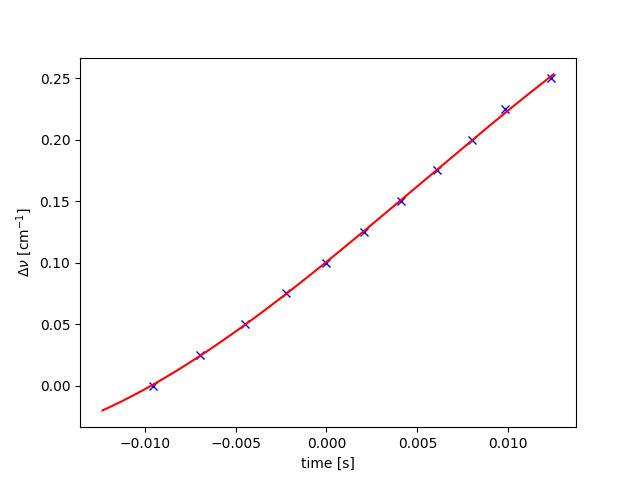
\includegraphics[scale = 0.5]{./absorbtion/frequencyCorrection}
\end{figure}

Die Frequenz des Lasers sei $\nu_0+\nu$, wobei $nu_0=\frac{c}{780\mathrm{nm}}$ die ungefäre Frequenz des Lasers ist. Es ist $\nu \ll \nu_0$.
Betrachte einen Übergang mit Energiedifferenz $h\nu_1$ und einer Linienform ohne Dopplerverbreiterung $L(\nu)$.  Die Absorbierte Intensität bei Laserfrequenz $\nu$ ist proportional zu

$$\int_{-\infty}^{\infty} dv f_{MB}(v)L(\nu\sqrt{1-v/c}) \approx \int_{-\infty}^{\infty} dv f_{MB}(v)L(\nu_0+\nu-\nu_0 v/(2c))$$

Die Näherung ist gerechtfertigt, da für thermische Geschwindigkeiten $v \ll c$ und weil $\nu \ll \nu_0$. Da $L$ scharf um $\nu_0 + \nu_1$ gepeakt ist, kann man $L$ als Delta-Funktion approximieren. Die absorbierte Intensität ist daher proportional zu

$$f_{MB}(2c(\nu-\nu_1)/\nu_0) \sim e^{-mc^2(\nu-\nu1)^2/(2k_BT\nu_0^2)}$$

Für $N$ Übergänge bei Frequenzen $\nu_0+\nu_1,...,\nu_0+\nu_N$ lautet die Formel für die gemessene Intensität an der Photodiode also

\begin{equation}
I(\nu) = I_0(\nu) - \sum_{n=1}^N I_n e^{-mc^2(\nu-\nu_n)^2/(2k_BT\nu_0^2)}
\label{AbsorbtionFit}
\end{equation}

Da man mit den Messdaten nicht die Übergänge von einem s-Hyperfeinniveau zu verschiedenen p-Hyperfeinniveaus unterscheiden kann, fassen wir alle Übergänge, die vom selben s-Hyperfeinniveau ausgehen zu einem zusammen. Wir fitten (\ref{AbsorbtionFit}) an die Messdaten. Dabei verwenden wir für $I_0$ ein Polynom zweiter Ordnung.

\begin{figure}[h]
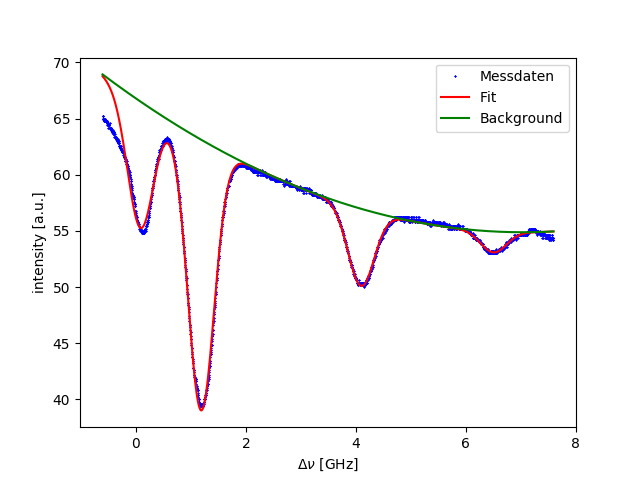
\includegraphics[scale = 0.5]{./absorbtion/fit.png}
\end{figure}

Die Abweichung des Fits an der linken Seite führen wir auf die Nichtlinearität des Durchstimmen des Lasers zurück. Der Fit weicht an der linken Seite nur vor dem ersten Peak des Referenzresonators ab. Unsere Interpolation von oben kann augenscheinlich nicht verwendet werden, um die Frequenz-Zeit Abhängigkeit links des ersten Peaks des Referenzresonators zu extrapolieren. Auch beim Experiment wurde beobachtet, dass der Laser in einem Frequenzbereich annähernd linear durchgestimmt wird, an den Rändern aber sehr nichtlinear.

Wir erhalten folgende Werte:

\begin{align*}
\nu_1 &= 0.082 \pm 0.001 GHz \\
\nu_2 &= 1.1854 \pm 0.0003 GHz \\
\nu_3 &= 4.094 \pm 0.002 GHz\\
\nu_4 &= 6.501 \pm 0.005 GHz \\
T&=350 \pm 2 K
\end{align*}

Damit ergeben sich die Abstände im Termschema zu $1.103 \pm 2 GHz$,  $2.909 \pm 0.003 GHz$ und $6.419 \pm 0.006 GHz$. Die Abweichungen zu den Literaturwerten können zu Teil damit erklärt werden, dass nicht klar ist, zu welchem p-Niveau die Übergänge sind, und dass wir die beziehung der p-Hypserfeinniveaus von Rb-85 und Rb-87 nicht kennen. ({\color{red}Edward: Hier auf jeden Fall weiter ausführen})

\section{Sättigungsspektroskopie}

Betrachte Übergänge wie oben. Der vom Pumpstrahl mit Frequenz $\nu_0+\nu$ angeregte Anteil der Atome mit Geschwindigkeit $v$ beträgt beträgt

$$n(\nu, v) = \sum_{i=1}^N A_i L_i(\nu_0+\nu-\nu_0 v/(2c))$$

mit Konstanten $A_1, ..., A_N$. Die gemessene Intensität beträgt dann

$$I(\nu) = I_0(\nu)-\int_{-\infty}^{\infty} f_{MB}(v)(1-n(\nu, v))\sum_{j=1}^N B_j L_i(\nu_0+\nu+\nu_0 v/(2c))$$

Mit Konstanten $B_1, ..., B_N$ und Ausgangsintensität $I_0(\nu)$. Erste Summand im Integraten ist der selben Term wie bei der Absorbtionsspektroskopie. Den zweiten Term nähern wir, indem wir ausnutzen, dass  $L_i(\nu_0+\nu-\nu_0 v/(2c)) L_j(\nu_0+\nu+\nu_0 v/(2c))$ nur für $v \approx 2c \frac{\nu_i-\nu}{\nu_0}$ nicht verschwindend ist. Deshalb können wir $f_{MB}(v)$ als konstant annehmen und haben nur noch den Term

$$T_{ij}=\int_{-\infty}^\infty dv L_i(\nu_0+\nu-\nu_0 v/(2c)) L_j(\nu_0+\nu+\nu_0 v/(2c))$$

Sei $L_\gamma$ die Lorenzverteilung um 0 mit FWHM $\gamma$. Wir nehmen $L_i(x) = L_{\gamma_i}(x-(\nu_0+\nu_i)$ and. Dann ist

\begin{align*}
T_{ij} &= \frac{2c}{\nu_0}\int_{-\infty}^\infty du L_{\gamma_i}(2\nu-(\nu_i+\nu_j)-u)L_{\gamma_j}(u)\\
&= \frac{2c}{\nu_0} (L_{\gamma_i} * L_{\gamma_j})(2\nu-(\nu_i+\nu_j)) \\
&= \frac{2c}{\nu_0} L_{\gamma_i+\gamma_j}(2\nu-(\nu_i+\nu_j)) \\
\end{align*}

Damit ergibt sich eine insgesamt Fitfunktion
\begin{equation}
I(\nu) = I_0(\nu)-\sum_{i=1}^N B_i e^{-mc^2(\nu-\nu_i)^2/(2k_BT\nu_0^2)} +\sum_{\substack{i,j=1\\i\leq j}}^N C_{ij} L_{\gamma_i+\gamma_j}(2\nu-(\nu_i+\nu_j))
\label{SaettigungsFit1}
\end{equation}


mit Konstanten $C_{ij}$. Wir haben $T_{ij}=T_{ji}$ ausgenutzt.\\

Wir haben jeden der vier großen Peaks individuell gefittet. Ein fitten mit der Funktion aus (\ref{SaettigungsFit1}) war jedoch leider nicht möglich, der Fit ist nicht konvergiert. Wir führen das darauf zurück, dass die Variation der $B_i$ die Funktion kaum verändert, solange ihre Summe konstant bleibt. Stattdessen haben wir, wie bei der Absorbtionsspektroskopie, die Gausspeaks zu einem einzelnen zusammengefasst und mit der Funktion

 \begin{equation}
I(\nu) = I_0(\nu)-B e^{-mc^2(\nu-\nu_{Gauss})^2/(2k_BT\nu_0^2)} +\sum_{\substack{i,j=1\\i\leq j}}^N C_{ij} L_{\gamma_i+\gamma_j}(2\nu-(\nu_i+\nu_j))
\label{SaettigungsFit2}
\end{equation}

gefittet. $I_0$ haben wir als Polynom ersten Grades gefittet. Die weiteren Fit Parameter sind $B$, $\nu_{Gauss}$, $T$, $C_{ij}$ und $\gamma_i$. Das Ergebnis der Fits mit und ohne Dopplerhintergrund ist hier dargestellt:

\begin{figure}[h]
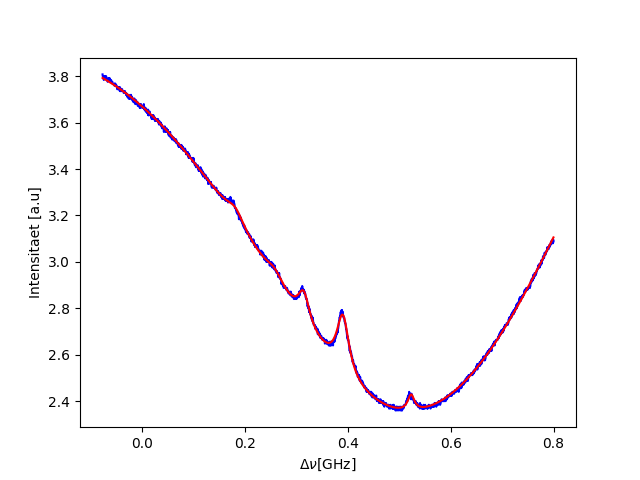
\includegraphics[scale = 0.5]{./saturation/peak1/fit.png}
\end{figure}

\begin{figure}[h]
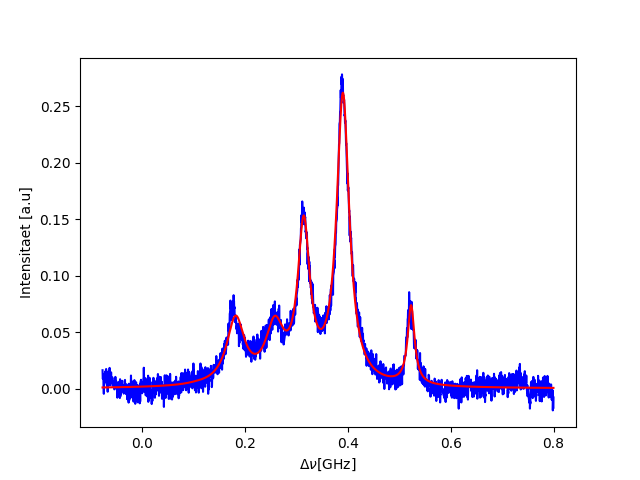
\includegraphics[scale = 0.5]{./saturation/peak1/gaussCorrected.png}
\end{figure}

\begin{figure}[h]
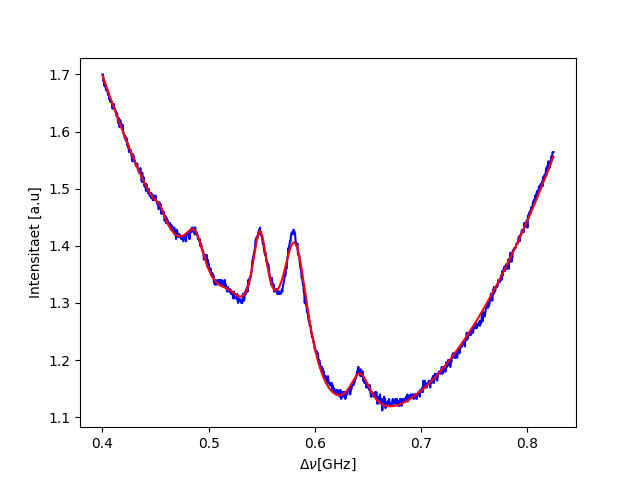
\includegraphics[scale = 0.5]{./saturation/peak2/fit.png}
\end{figure}

\begin{figure}[h]
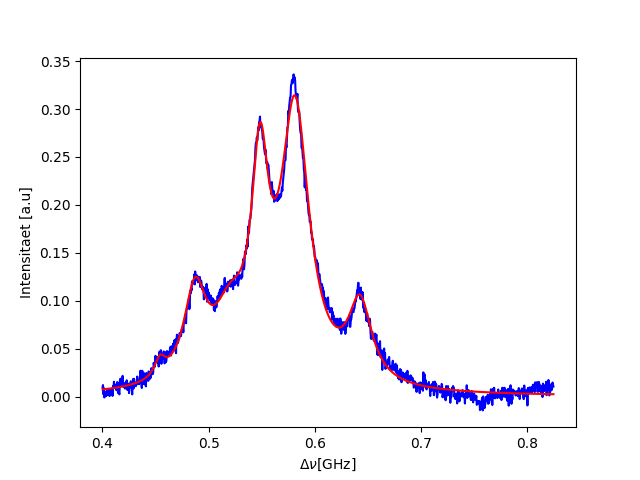
\includegraphics[scale = 0.5]{./saturation/peak2/gaussCorrected.png}
\end{figure}

\begin{figure}[h]
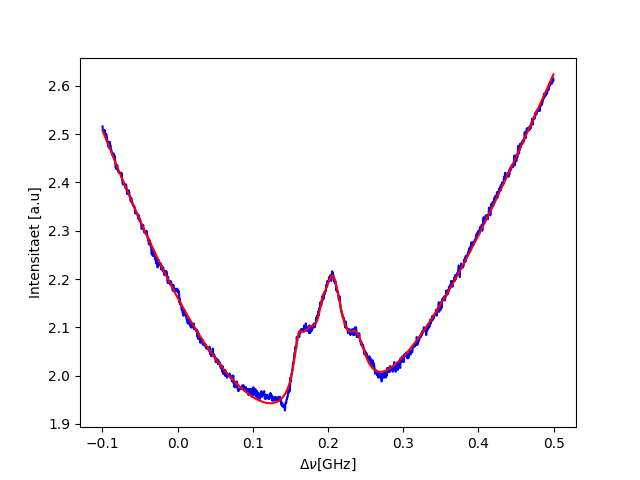
\includegraphics[scale = 0.5]{./saturation/peak3/fit.png}
\end{figure}

\begin{figure}[h]
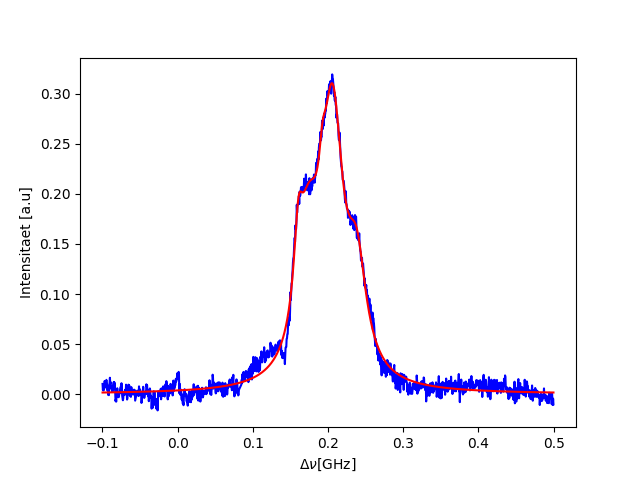
\includegraphics[scale = 0.5]{./saturation/peak3/gaussCorrected.png}
\end{figure}

\begin{figure}[h]
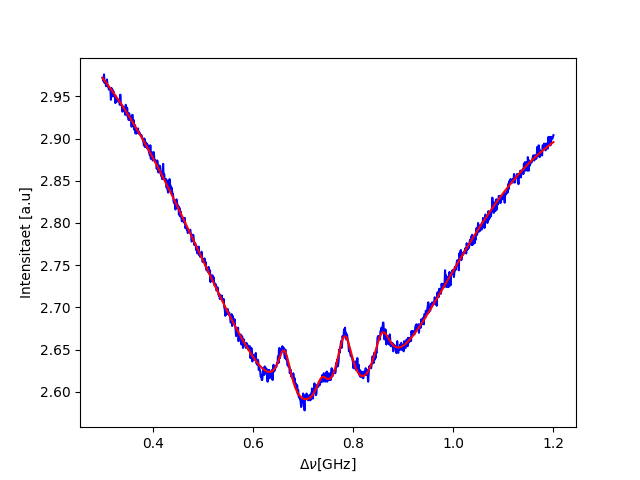
\includegraphics[scale = 0.5]{./saturation/peak4/fit.png}
\end{figure}

\begin{figure}[h]
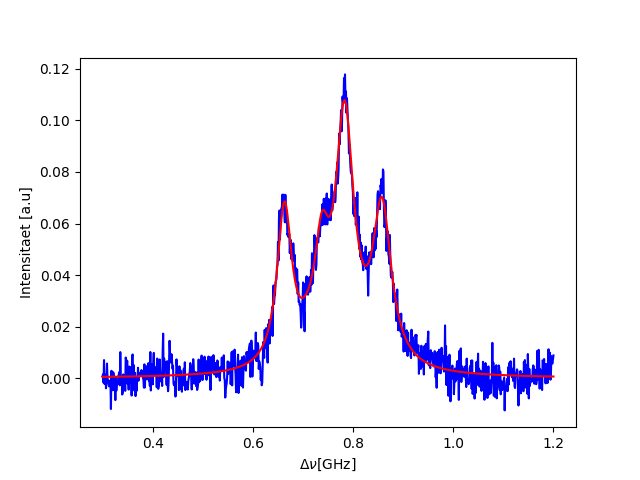
\includegraphics[scale = 0.5]{./saturation/peak4/gaussCorrected.png}
\end{figure}

Wir erhalten folgende Frequenzen:

Übergänge von Rb 87 von $F=2$:

\begin{align*}
\nu_{F'=1} &= 105.7 \pm 0.4 MHz \\
\nu_{F'=2} &= 257.9 \pm 0.3 MHz \\
\nu_{F'=3} &= 523.1 \pm 0.2 MHz  
\end{align*}

Übergänge von Rb 85 von $F=3$:

\begin{align*}
\nu_{F'=2} &= 454.2 \pm 0.3 MHz \\
\nu_{F'=3} &= 520.6 \pm 0.3 MHz \\
\nu_{F'=4} &= 642.7 \pm 0.2 MHz  
\end{align*}

Übergänge von Rb 85 von $F=2$:

\begin{align*}
\nu_{F'=1} &= 147.0 \pm 0.5 MHz \\
\nu_{F'=2} &= 174.1 \pm 0.5 MHz \\
\nu_{F'=3} &= 238.2 \pm 0.3 MHz  
\end{align*}

Übergänge von Rb 87 von $F=1$:

\begin{align*}
\nu_{F'=0} &= 617.4 \pm 0.8 MHz \\
\nu_{F'=1} &= 708.6 \pm 0.7 MHz \\
\nu_{F'=2} &= 857.8 \pm 0.5 MHz  
\end{align*}

Damit ergeben sich die Differenzen zwischen den Niveaus zu $122.1 \pm 0.5 MHz$, $66.4 \pm 0.6MHz$ bzw. $64.1 \pm 0.8 MHz$ und $28 \pm 1 MHz$ für Rb 85 sowie $265.2 \pm 0.5 MHz$, $152.2 \pm 0.7 MHz$ bzw. $149 \pm 2 MHz$ und $91 \pm 2 MHz$. ({\color{red} Edward: Etwas zu den Fehlern schreiben, insb. zu dem großen Fehlen (91 MHz vs. 72 MHz) bei der letzten Differenz.})\\

Man  kann nun noch Versuchen, die Abstände der s-Hyperfeinniveaus beider Isotope genauer bestimmt, indem man mit $\nu_{Gauss} - \nu_i$ korrigiert ({\color{red} Edward: Bitte genauer erklären}). Man erhält
$3.07 \pm 0.01 GHz$ bzw $3.10 \pm 0.02 GHz$ für Rb-85 und $6.51 \pm 0.01 GHz$ bzw $6.68 \pm 0.02 GHz$. {\color{red}Wo kommen die Abweichungen bei Rb 87 her?} 

\end{document}

